\chapter{Extension to 3D} \label{chap:MahdadMethod3d}

This thesis suggests to blend crossline sources, i.e. in combination with the movement of the seismic vessel one effectively blends sources in 3D.

The deblending method of \citet{Mahdad-Deblending-Method} is designed for 2D blended data. In principle, each step of the method can be applied to 3D data as well. In this thesis I will extend the deblending method of \citet{Mahdad-Deblending-Method} to 3D and demonstrate its performance.

First, the data sorting will be modified such that the blended 3D data can be described using the same forward model as in section \ref{sec:Ch-Theory-Operator}. Second, the $f$-$k$-filter will be extended to remove noise in crossline and inline direction. The presented data sorting will allow to maintain all other steps of the deblending algorithm of \citet{Mahdad-Deblending-Method} unchanged.

\section{Data Sorting} \label{sec:Ch-Theory-3dExtension-DataSorting}

\subsection*{Data Matrix}

In 3D acquisition the sources and receivers are distributed on a 2D surface. Thus, their locations are defined by their crossline and inline positions, ($x$, $y$). Each data point which is measured by a source receiver pair at a specific time is therefore constraint by 5 coordinates: Time $t$, receiver crossline and inline position ($x_r$, $y_r$), and source crossline and inline position ($x_s$, $y_s$).

Before applying the Mahdad deblending method the 5D data array will be reorganized in a 2D data matrix according to \citet{Delphi-Format}. For this data sorting a 1D Fourier transform with respect to time is performed and a frequency slice is selected. This reduces the data array from 5 to 4 dimensions. 

The 4D data array is sorted in a 2D matrix data matrix, $\mathbf{P}$, with as many rows as receivers and as many columns as sources. The total number of receivers (or sources) is obtained by multiplying the number of crossline and inline receivers (or sources). Assume there are $Ns_x$ sources per crossline. The sources of the first crossline are assigned to the first $Ns_x$ columns of the data matrix, the sources of the second crossline are assigned to the next $Ns_x$ columns of the data matrix, etc. The cross- and inline receivers are sorted in the rows of the data matrix in analogy. This is illustrated in Figure \ref{fig:Ch-Theory-DelphiFormat} and \ref{fig:Ch-Theory-DataSorting}. 

\begin{figure}
	\centering
	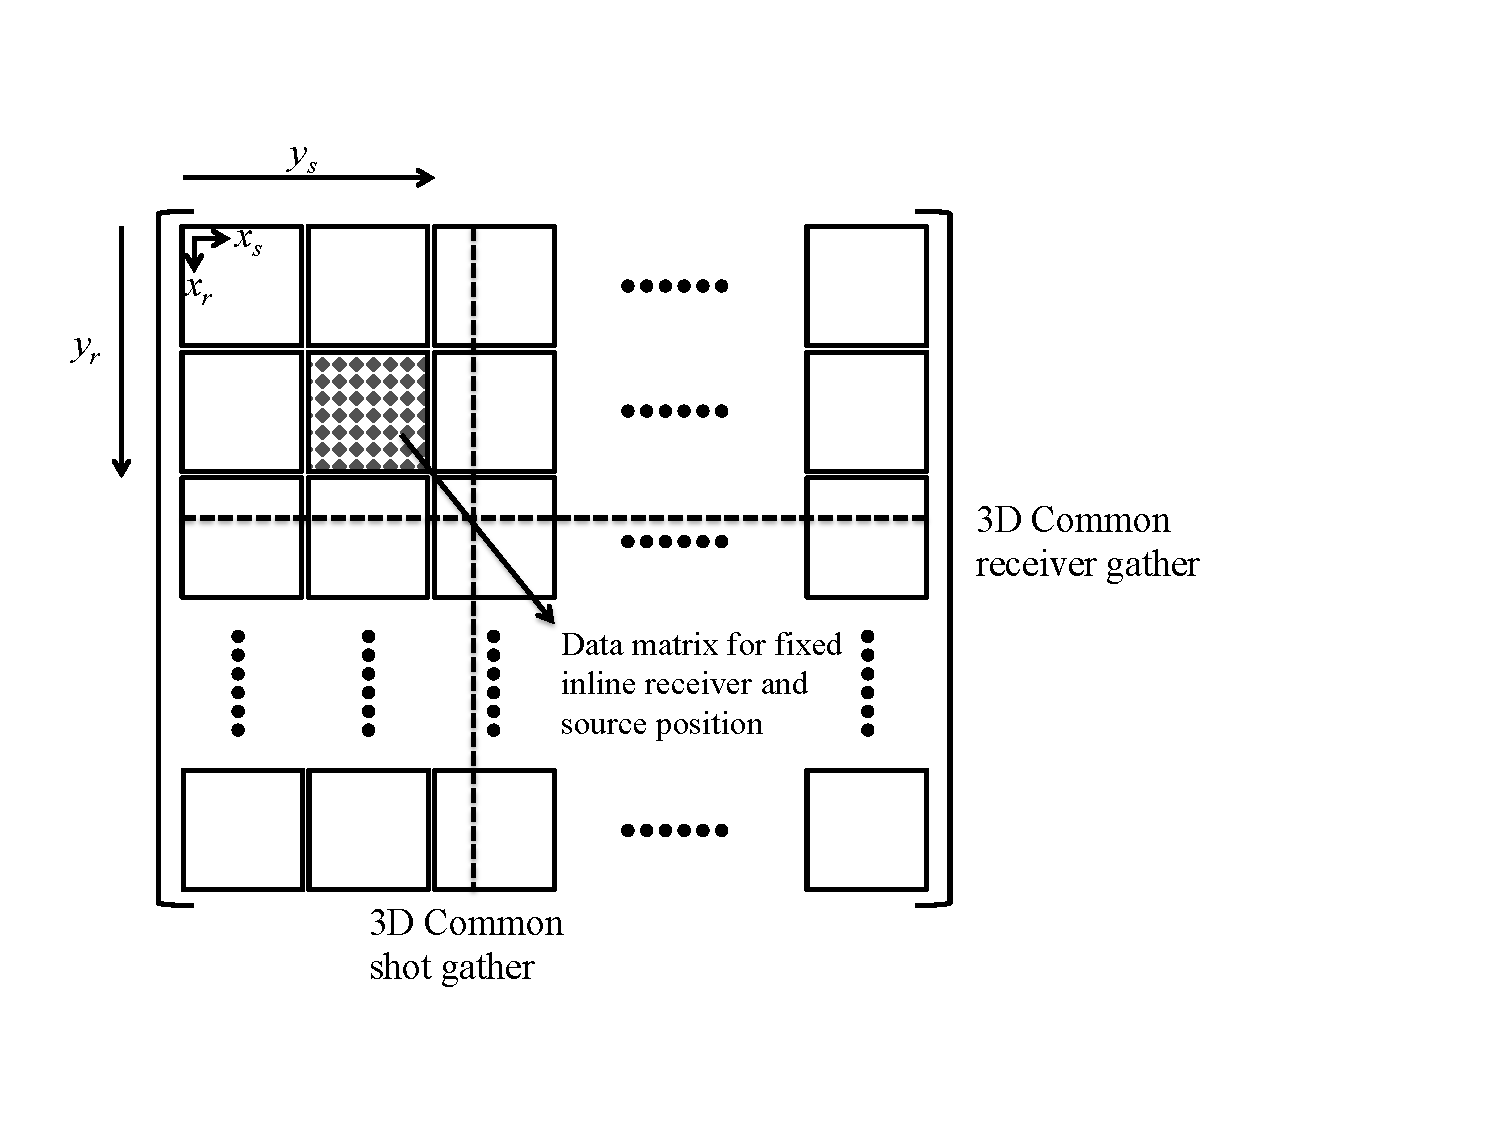
\includegraphics[width=0.6\textwidth]{Plots/DelphiFormat-v2}
	\caption{Illustration of the data matrix $\mathbf{P}$ for 3D data \citep{Delphi-Format}. $y_r$ and $y_s$ represent the inline receiver and source positions. $x_r$ and $x_s$ represent the crossline receiver and source positions. Each row refers to a 3D common receiver gather and each column to a 3D common shot gather. A sub-matrix with fixed receiver and source inline positions ($y_r$, $y_s$) is equivalent to a data matrix for 2D acquisition.}
	\label{fig:Ch-Theory-DelphiFormat}
\end{figure}


\begin{figure}
	
	\begin{subfigure}[t]{\textwidth}
	 	\centering
		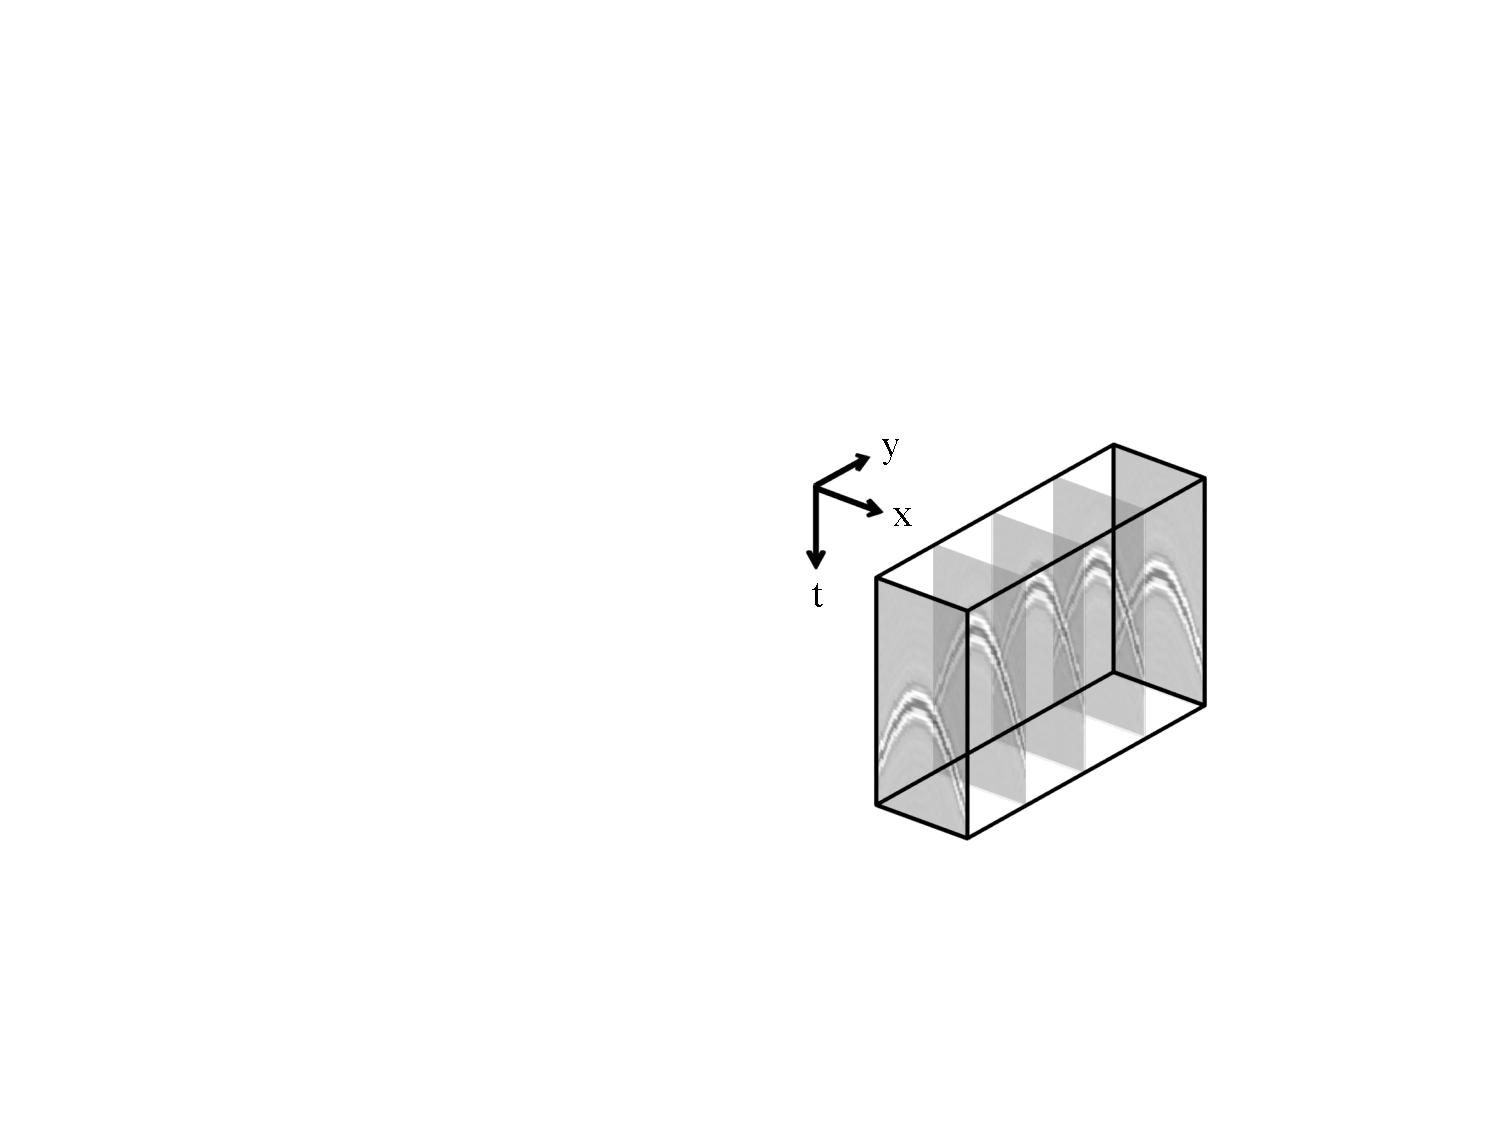
\includegraphics[width = 0.3\textwidth]{Plots/data3d}
		\caption{}
		\label{fig:Ch-Theory-Data3d}
	\end{subfigure}
	\par\bigskip
	\begin{subfigure}[t]{\textwidth}
		\centering
		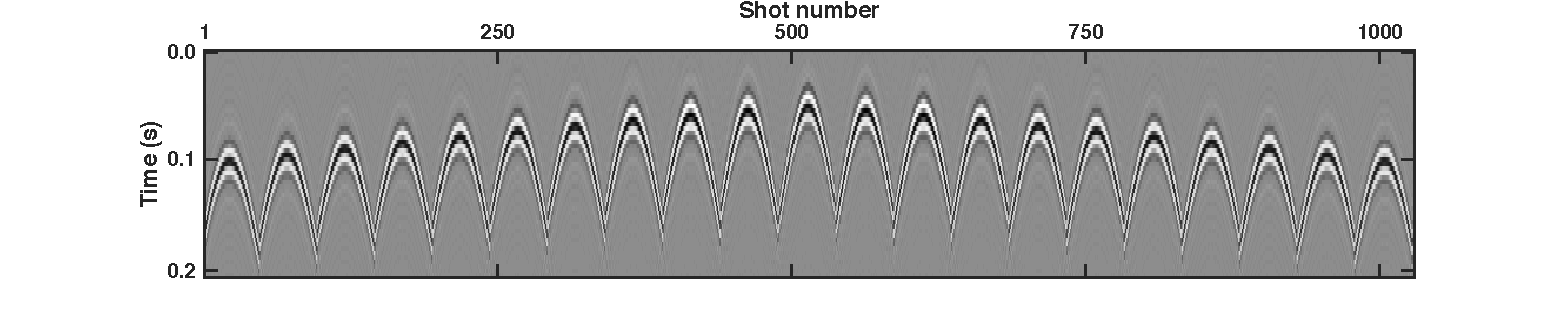
\includegraphics[width = \textwidth]{Plots/data3d_Delphi}
		\caption{}
		\label{fig:Ch-Theory-Data3d_Delphi}
	\end{subfigure}
	
	\caption{(a) Common receiver gather of a 3D data set with crossline (x) and inline (y) sources. (b) Resorted data set. Individual crossline sections are plotted next to each other in 2D.}
	\label{fig:Ch-Theory-DataSorting}
\end{figure}


\subsection*{Blending matrix}

As described in section \ref{sec:BlendingMatrix} each row of the blending matrix, $\mathbf{\Gamma}$, captures one source. For extension to 3D the sources of the first crossline are saved in the top $Ns_x$ rows of the blending matrix, followed by the sources of the second crossline etc. (see Figure \ref{fig:Ch-Theory-3D-BlendingMatrix-Design}). This framework allows to blend any source combination independent of the cross- and inline positions of the involved sources.

With the new data and blending matrix sorting one can already apply the 2D Mahdad method to the 3D data.

\begin{figure}

	\begin{subfigure}[t]{0.5\textwidth}
		\centering
		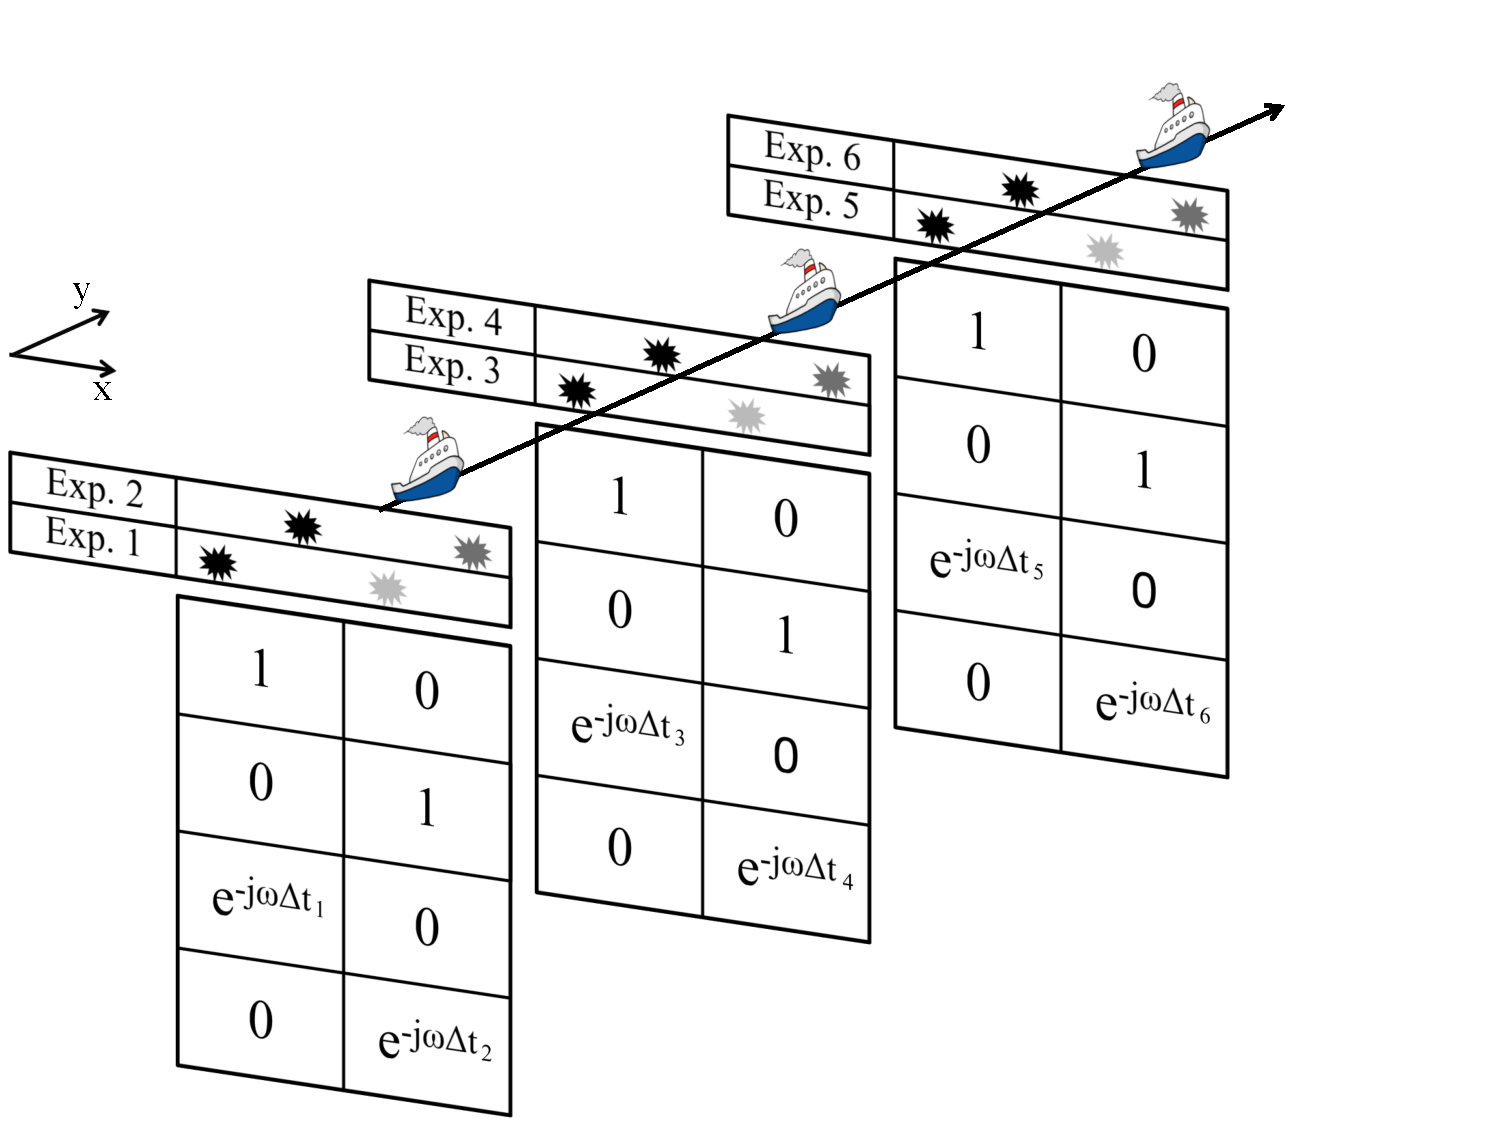
\includegraphics[width = \textwidth]{Plots/DrawingsCartesianFormat1}
		\caption{}
		\label{fig:Ch-Theory-3D-BlendedAcquisition}
	\end{subfigure}
	%
	\begin{subfigure}[t]{0.5\textwidth}
		\centering
		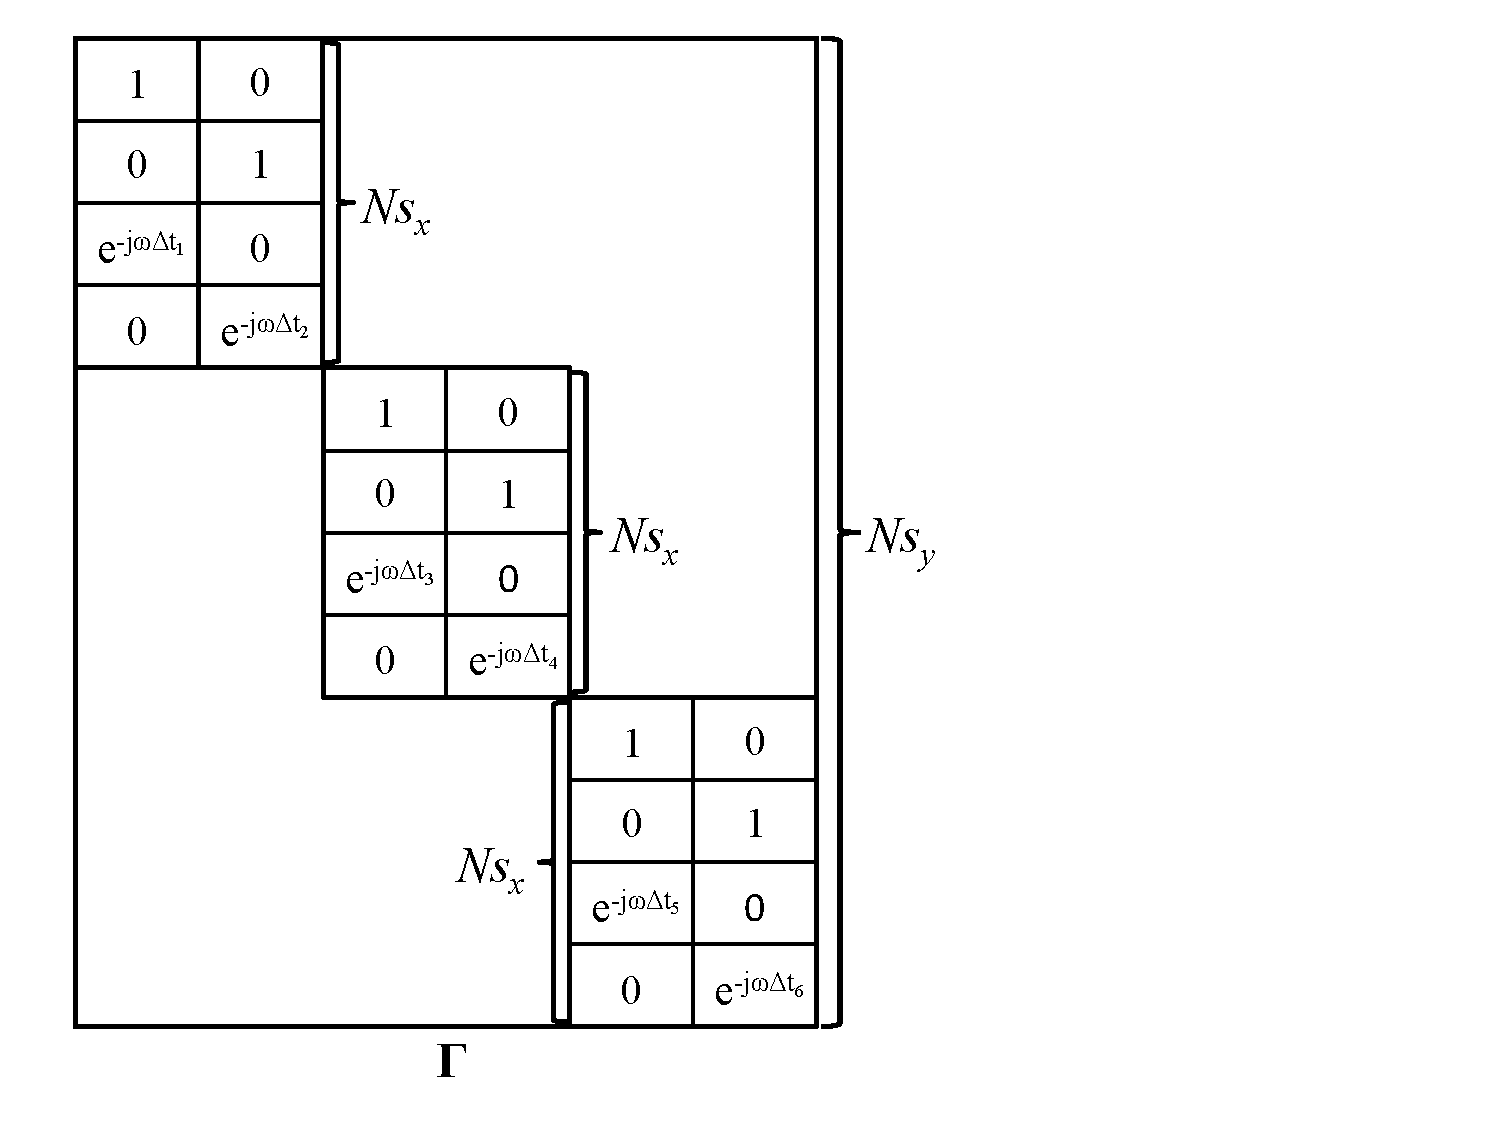
\includegraphics[width = 0.7\textwidth]{Plots/DrawingsCartesianFormat2}
		\caption{}
		\label{fig:Ch-Theory-3D-BlendingMatrix}
	\end{subfigure}
	
	\caption{Illustration of the blending matrix, $\mathbf{\Gamma}$, for 3D acquisition. (a) At each of the $Ns_y$ inline position the crossline sources ($x$ direction) are blended. Each of these 2D blending processes is described by a 2D blending matrix, which has as many rows as there are crossline sources, $Ns_x$. (b) The 2D blending matrices are assembled in a single 3D blending matrix, $\mathbf{\Gamma}$, which has $Ns_x$ by $Ns_y$ rows.}
	\label{fig:Ch-Theory-3D-BlendingMatrix-Design}

\end{figure}

\section{3D FKK Filter} \label{sec:Ch-Theory-3dExtension-FKK}

In section \ref{sec:IterBlenNoiseEst} the 2D $f$-$k$ filter was introduced. In 3D there are two spatial direction ($x$, $y$), i.e. the filter can be extended to a 3D $f$-$k_x$-$k_y$-filter.

One obtains the $f$-$k_x$-$k_y$-spectrum by applying an n-dimensional Fourier transform to the 5D data array. As Mahdad's deblending method is applied to common receiver gathers one picks a single receiver, i.e constant cross- and inline receiver number. Next, a constant frequency slice is selected. This leaves a 2D matrix, which captures the cross- and inline wavenumbers ($k_x$, $k_y$) (see Figure \ref{fig:Ch-Theory-FK-f_slice-data}). Again the minimum velocity, $v_{min}$, and the frequency, $f$, determine the maximum wavenumber, $k_{max}$, according to equation \ref{eq_Ch-Theory-MaxWavenmber}. The total wavenumber, $k_{T}$, must be smaller than the maximum wavenumber, $k_{max}$,

\begin{equation}
	k_{T} = \sqrt{k_x^2 + k_{y}^2} < k_{max}.
	\label{eq:Ch-Theory-TotalWavenumber}
\end{equation}

Hence the signal "cone" is defined by a circle (see Figure \ref{fig:Ch-Theory-FK-f_slice-mask}). This is repeated for each frequency component, such that the overall $f$-$k_x$-$k_y$-mask is a 3D cone. Finally, this mask is computed for each receiver gather.

Once the mask is built for a 5D data array it can either be applied to filter a 5D data array, or the mask is sorted to 2D according to section \ref{sec:Ch-Theory-3dExtension-DataSorting}, and applied to the $f$-$k_x$-$k_y$-spectrum of the data matrix (see Figure \ref{fig:Ch-Theory-FK-delphi-data}, \ref{fig:Ch-Theory-FK-delphi-mask}).

\begin{figure}
	\centering
	\begin{subfigure}[t]{0.45\textwidth}
		\centering
		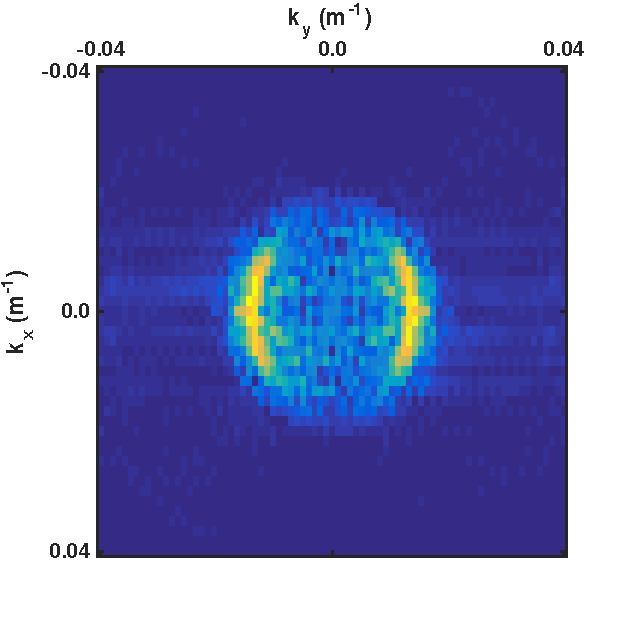
\includegraphics[width=0.6\textwidth]{Plots/FK-mask/FK-f_slice-data}
		\caption{}
		\label{fig:Ch-Theory-FK-f_slice-data}
	\end{subfigure}
	%
	\centering
	\begin{subfigure}[t]{0.45\textwidth}
		\centering
		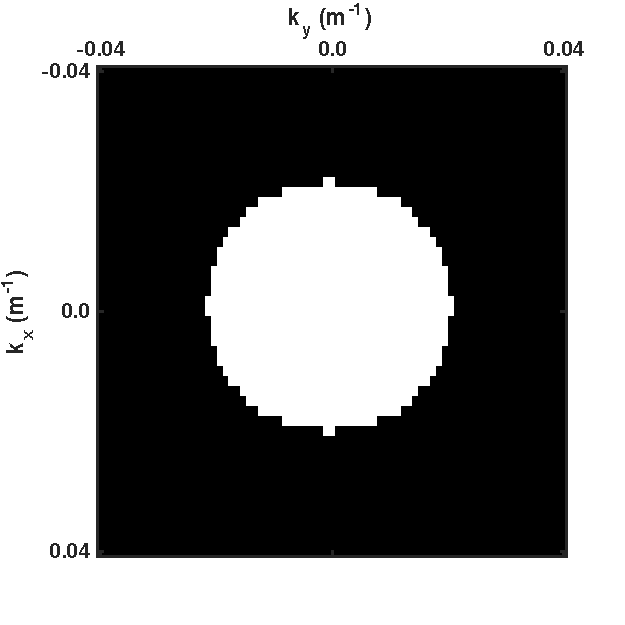
\includegraphics[width=0.6\textwidth]{Plots/FK-mask/FK-f_slice-mask}
		\caption{}
		\label{fig:Ch-Theory-FK-f_slice-mask}
	\end{subfigure}
	
	\begin{subfigure}[t]{\textwidth}
		\centering
		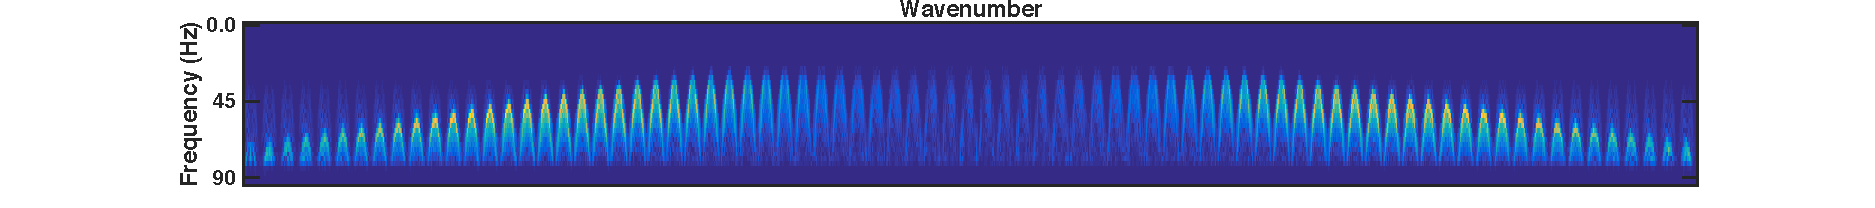
\includegraphics[width=0.9\textwidth]{Plots/FK-mask/FK-delphi-data}
		\caption{}
		\label{fig:Ch-Theory-FK-delphi-data}
	\end{subfigure}
	\par\bigskip
	\begin{subfigure}[t]{\textwidth}
		\centering
		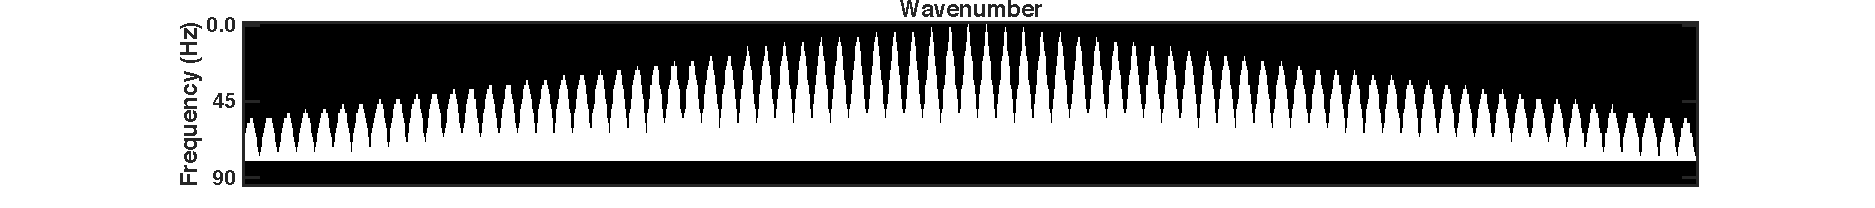
\includegraphics[width=0.9\textwidth]{Plots/FK-mask/FK-delphi-mask}
		\caption{}
		\label{fig:Ch-Theory-FK-delphi-mask}
	\end{subfigure}
	
	\caption{Illustration of the 3D $f$-$k_x$-$k_y$-filter. (a) and (b) show a \SI{30}{\hertz} frequency slice of the $f$-$k_x$-$k_y$-spectrum, where $k_x$ and $k_y$ refer to the crossline and inline wavenumber respectively. (a) is the spectrum of the data in Figure \ref{fig:Ch-Theory-Data3d_Delphi}, and (b) is the corresponding filter mask. The white area equals 1 and the black area is 0. (c) and (d) display the $f$-$k_x$-$k_y$-spectrum sorted according to section \ref{sec:Ch-Theory-3dExtension-DataSorting}.  Note that the sorting implies that the wavenumber axis is a mix of crossline and inline wavenumbers. For this reason the wavenumber axis has no labels. (c) represents the data and (d) the filter mask.}
	\label{fig:Ch-Theory-FKK-Mask}

\end{figure}